\documentclass[a4paper,12pt,french]{article}

\usepackage[cours]{../../Style}



% Début du document
%%%%%%%%%%%%%%%%%%%
\begin{document}

\title{Fonctions: Généralités}
\maketitle

\begin{programme}
\item Fonctions à valeurs réelles définies sur un intervalle ou une réunion finie d'intervalles
\item Courbe représentative: $(x,f(x))$ \ldots
\item Fonction paire, impaire. Traduction géométrique
\item Capacités:
\begin{itemize}
\item Exploiter l'équation d'une courbe: appartenance, coordonnées
\item Modéliser par des fonctions [ \ldots ]
\item Résoudre des (in)équations: graphiquement, algébriquement, tableaux de signes
\item Etudier la parité dans des cas simples
\end{itemize}
\end{programme}
%\begin{FlushLeft}

\section{Définitions, notations}

\begin{defin}
Soit $D \subset \R$. On appelle fonction $f$ sur l'ensemble $D$ le processus qui à tout nombre $x \in D$ associe un \textbf{unique} réel noté $f(x)$. On note $\fonction f D {\R} x {f(x)}$.
\begin{center}
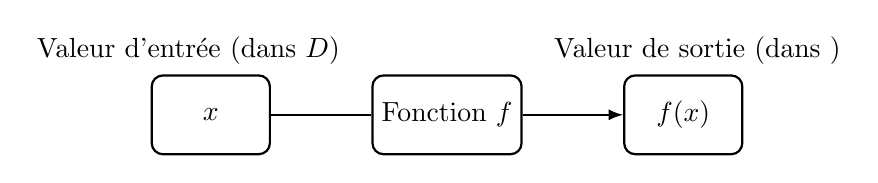
\begin{tikzpicture}[scale=1]
\node[draw,rectangle,thick, minimum height=10mm, minimum width=15mm, rounded corners] (x) at (-3,0) {$x$};
\node[anchor=south east,xshift=1cm] at (x.north east) {Valeur d'entrée (dans $D$)};
\node[draw,rectangle,thick, minimum height=10mm, minimum width=15mm, rounded corners] (f) at (0,0) {Fonction $f$};
\node[draw,rectangle,thick, minimum height=10mm, minimum width=15mm, rounded corners] (fx) at (3,0) {$f(x)$};
\node[anchor=south west,xshift=-1cm] at (fx.north west) {Valeur de sortie (dans $\R$)};
\draw[-,>=latex,thick] (x) to (f);
\draw[->,>=latex,thick] (f) to (fx);
\end{tikzpicture}
\end{center}

On dit alors que:
\begin{itemize}
\item $f(x)$ est l'image de $x$
\item $x$ est un antécédent de $f(x)$
\item $D$ est l'ensemble ( ou domaine ) de définition de $f$
\end{itemize}

\end{defin}

\begin{ex}
On définit la fonction $\fonction f {\R} {\R} x {x^2-x}$.
\begin{itemize}
\item L'ensemble de définition de $f$ est $\R$.
\item L'image de $2$ par la fonction $f$ est $2$: $f(2)=2^2-2=2$.
\item $2$ est un antécédent de $2$ par la fonction $f$. $-1$ en est aussi un car $f(-1)=(-1)^2+1=2$.
\end{itemize}
\end{ex}

\begin{rmq}
Chaque nombre dans $D$ possède une unique image, mais plusieurs antécédents d'un même nombre peuvent exister.
\end{rmq}

\section{Représentation graphique d'une fonction}

\begin{defin}
Dans un repère du plan, l'ensemble des points $(x,f(x))$ pour $x \in D$ constitue la courbe de $f$. L'équation de la courbe de $f$ est $y=f(x)$ pour $x \in D$.
\end{defin}

\begin{methode}
Dans la pratique, il faut placer plusieurs points pour tracer la courbe d'une fonction le plus précisément possible. On peut s'aider d'une table de valeurs.
\end{methode}

\begin{ex}
\begin{center}
\begin{tabularx}{0.95\linewidth}{ 
  | >{\centering\arraybackslash}c 
  | >{\centering\arraybackslash}X
  | >{\centering\arraybackslash}X
  | >{\centering\arraybackslash}X
  | >{\centering\arraybackslash}X
  | >{\centering\arraybackslash}X
  | >{\centering\arraybackslash}X
  | >{\centering\arraybackslash}X
  | >{\centering\arraybackslash}X
  | >{\centering\arraybackslash}X| } \hline
$x$ & $-1.5$ & $-1$ & $-0.5$ & $0$ & $0.5$ & $1$ & $1.5$ & $2$ & $2.5$ \\ \hline
$f(x)$ & & & & & & & & &\rule[-7pt]{0pt}{30pt} \\ \hline
\end{tabularx}
\end{center}

\begin{center}
\begin{tikzpicture}
\begin{axis}[
styleglobal,
width=0.8*\linewidth,
xmin=-4, xmax=4,
ymin=-1, ymax=4,
xtick distance=1,
ytick distance=1,
]
\addplot[styleplot] {x^2-x} node [pos=0.85,right] {$\mathscr C_f$};
\addlegendentry{$f(x)=x^2-x$};
\pgfplotsinvokeforeach{-1.5,-1,...,2.5}{\node[stylepoint,fill=red] at (#1,#1*#1-#1) {};}
\draw[color=blue,dashed,very thick] (2.2, 0) -- (2.2, 2.2^2-2.2) node [pos=0,below] {$x$};
\draw[color=blue,dashed,very thick] (2.2, 2.2^2-2.2) -- (0, 2.2^2-2.2) node [pos=1,left] {$f(x)$};
\node[stylepoint,fill=blue] at (2.2,2.2^2-2.2) {};
%\addplot +[mark=none,color=red,style=dashed,very thick] coordinates {(-1, 0) (-1, 2)};
%\addplot +[mark=none,color=red,style=dashed,very thick] coordinates {(-1, 2) (0, 2)};
%\node[label={0:{$(0,1)$}},rectangle,fill,inner sep=2pt] at (axis cs:0,1) {};
%\node[label={[label distance=2pt]-90:{$(0,1)$}},rectangle,fill,inner sep=0pt, minimum height=0pt, minimum width=4pt] at (axis cs:1,1) {};
\end{axis}
\end{tikzpicture}
\end{center}

Les points de coordonnées $(-1;2)$ et $(1;0)$ appartiennent à la courbe de $f$, mais pas le point de coordonnées $(0;1)$.

\end{ex}

\section{Résolution graphique d'équations}

\subsection{Equations du type $f(x)=k$}

\begin{methode}
\begin{center}
\begin{tabularx}{1\linewidth}{|X|X|} \hline
\Centering{
\begin{tikzpicture}[scale=1]
\begin{axis}[
axis x line=bottom,
axis y line = left,
axis lines=middle,
width=1.1*\linewidth,
height=0.75*\linewidth,
xmin=-0.5, xmax=4.5,
ymin=-0.5, ymax=4,
enlargelimits={abs=0.2},
xlabel={$x$},
ylabel={$y$},
%ytick distance=1,
ticks=none,
grid style=dashed,
%axis equal,
legend pos=north east,
xlabel style={at={(ticklabel* cs:0.95)},below=0.1},
]
\addplot[samples=101,smooth,ultra thick,domain=(-2:5),mark=none]{3.5*e^(-0.4*(x-2)^2)} node [pos=0.75,right] {$\mathscr C_f$};

\addplot +[mark=none,color=blue,style=dashed,very thick] coordinates {(-1,2.8) (5, 2.8)} node [pos=0.18,above right] {$k$};
\node[circle, minimum size=1pt,fill,color=blue,inner sep=2pt] at (axis cs:1.25,2.8) {};
\node[circle, minimum size=1pt,fill,color=blue,inner sep=2pt] at (axis cs:2.75,2.8) {};
\addplot +[mark=none,color=blue,style=dashed,very thick] coordinates {(1.25,0) (1.25, 2.8)} node [pos=0,below] {$a$};
\addplot +[mark=none,color=blue,style=dashed,very thick] coordinates {(2.75,0) (2.75, 2.8)} node [pos=0,below] {$b$};
%\addplot +[mark=none,color=red,style=dashed,very thick] coordinates {(-1, 0) (-1, 2)};
%\addplot +[mark=none,color=red,style=dashed,very thick] coordinates {(-1, 2) (0, 2)};
%\node[label={0:{$(0,1)$}},rectangle,fill,inner sep=2pt] at (axis cs:0,1) {};
%\node[label={[label distance=2pt]-90:{$(0,1)$}},rectangle,fill,inner sep=0pt, minimum height=0pt, minimum width=4pt] at (axis cs:1,1) {};
\end{axis}
\end{tikzpicture}}
&
Résoudre l'équation $f(x)=k$ signifie trouver les antécédents de $k$ par la fonction $f$.

Cela revient donc à chercher l'abscisse des points de la courbe dont l'ordonnée est $k$.

Ici, l'ensemble des solution de l'équation est:$$S=\{a;b \}$$ \vspace{-5mm}\\ \hline
\end{tabularx}
\end{center}
\end{methode}

\begin{exs}
\begin{center}
\begin{tabularx}{1\linewidth}{|Y|Y|Y|} \hline
\begin{tikzpicture}
\begin{axis}[
styleglobal,
width=0.9*\linewidth,
xmin=-5, xmax= 5,
ymin=-2, ymax=5,
xtick distance=1,
ytick distance=1,
minor x tick num=0,
minor y tick num=0,
%tick label style = {font=\scriptsize},
]
\addplot[styleplot] plot coordinates {(-4,2) (-2,-1) (0,0) (2,3) (4,0.5)};
\end{axis}
\end{tikzpicture}
&
\begin{tikzpicture}
\begin{axis}[
styleglobal,
width=0.9*\linewidth,
xmin=-2, xmax= 8,
ymin=-2, ymax=5,
xtick distance=1,
ytick distance=1,
minor x tick num=0,
minor y tick num=0,
%tick label style = {font=\scriptsize},
]
\addplot[styleplot] plot coordinates {(-1,4) (4,2) (5,4) (7,-1.5)};
\end{axis}
\end{tikzpicture}
&
\begin{tikzpicture}
\begin{axis}[
styleglobal,
width=0.9*\linewidth,
xmin=-7, xmax= 3,
ymin=-5, ymax=2,
xtick distance=1,
ytick distance=1,
minor x tick num=0,
minor y tick num=0,
%tick label style = {font=\scriptsize},
]
\addplot[styleplot] plot coordinates {(-6,1) (-3,-3) (-2,0) (2,-3.5)};
\end{axis}
\end{tikzpicture}
\\ \hline
Résoudre $f(x)=1$:
\rule[-1cm]{0pt}{1cm}
&
Résoudre $g(x)=1$:
\rule[-1cm]{0pt}{1cm}
&
Résoudre $h(x)=-4$:
\rule[-1cm]{0pt}{1cm} \\ \hline
\end{tabularx}
\end{center}
\end{exs}

\rem{Fiche, exos 1-2}

\subsection{Equations du type $f(x)=g(x)$}

\begin{methode}
\begin{center}
\begin{tabularx}{1\linewidth}{|X|X|} \hline
\Centering{
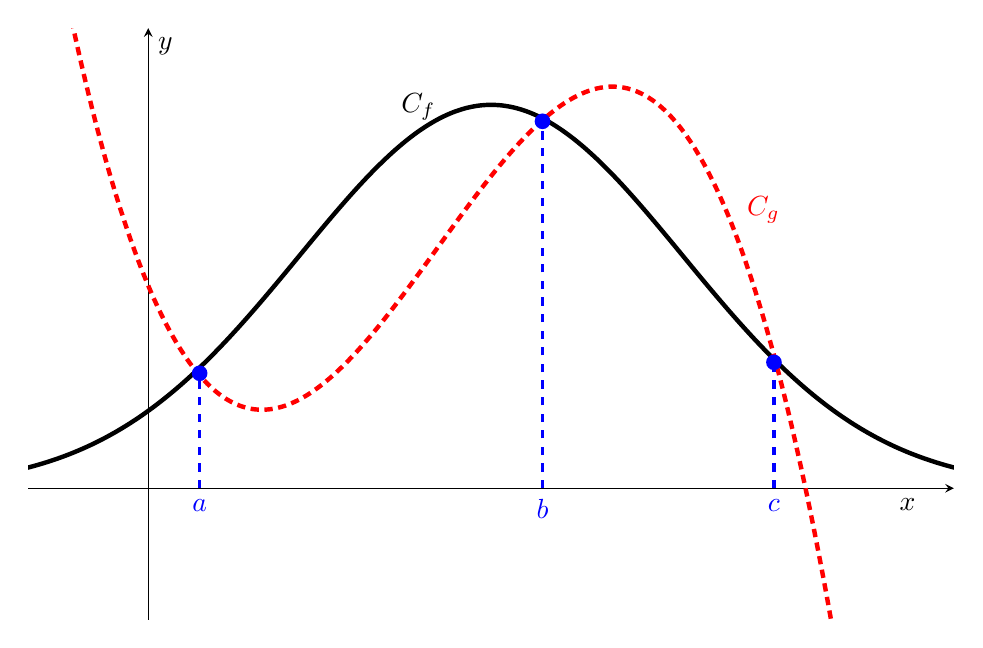
\begin{tikzpicture}[scale=1]
\begin{axis}[
axis x line=bottom,
axis y line = left,
axis lines=middle,
width=1.1*\linewidth,
height=0.75*\linewidth,
xmin=-0.5, xmax=4.5,
ymin=-1, ymax=4,
enlargelimits={abs=0.2},
xlabel={$x$},
ylabel={$y$},
ticks=none,
%ytick distance=1,
%axis equal,
yticklabel=\empty,
xticklabel=\empty,
xlabel style={at={(ticklabel* cs:0.95)},below=0.1},
]
\addplot[samples=101,smooth,ultra thick,domain=(-2:5),mark=none]{3.5*e^(-0.4*(x-2)^2)} node [pos=0.5,above] {$\mathscr C_f$};
\addplot[samples=101,smooth,ultra thick,domain=(-2:5),mark=none,color=red, densely dashed]{-0.69*x^3+3.49*x^2-3.72*x+1.85} node [pos=0.65,above right,color=red] {$\mathscr C_g$};

\addplot +[mark=none,color=blue,style=dashed,very thick] coordinates {(0.3,0) (0.3, 1.05)} node [pos=0,below] {$a$} node[pos=1,circle, minimum size=1pt,fill,inner sep=2pt] {};
\addplot +[mark=none,color=blue,style=dashed,very thick] coordinates {(2.3,0) (2.3, 3.35)} node [pos=0,below] {$b$} node[pos=1,circle, minimum size=1pt,fill,inner sep=2pt] {};
\addplot +[mark=none,color=blue,style=dashed,very thick] coordinates {(3.65,0) (3.65, 1.15)} node [pos=0,below] {$c$} node[pos=1,circle, minimum size=1pt,fill,inner sep=2pt] {};
%\addplot +[mark=none,color=red,style=dashed,very thick] coordinates {(-1, 0) (-1, 2)};
%\addplot +[mark=none,color=red,style=dashed,very thick] coordinates {(-1, 2) (0, 2)};
%\node[label={0:{$(0,1)$}},rectangle,fill,inner sep=2pt] at (axis cs:0,1) {};
%\node[label={[label distance=2pt]-90:{$(0,1)$}},rectangle,fill,inner sep=0pt, minimum height=0pt, minimum width=4pt] at (axis cs:1,1) {};
\end{axis}
\end{tikzpicture}}
&
Résoudre l'équation $f(x)=g(x)$ signifie trouver les nombres qui ont la même image par $f$ et $g$.

Cela revient donc à chercher l'abscisse des points d'intersection des deux courbes $\mathscr C_f$ et $\mathscr C_g$.

Ici, l'ensemble des solution de l'équation est:$$S=\{ a;b;c \}$$
\\ \hline

\end{tabularx}
\end{center}
\end{methode}

\begin{exs}
\begin{center}
\begin{tabularx}{\linewidth}{|Y|Y|Y|} \hline
\begin{tikzpicture}
\begin{axis}[
styleglobal,
width=0.9*\linewidth,
xmin=-5, xmax= 5,
ymin=-2, ymax=5,
xtick distance=1,
ytick distance=1,
minor x tick num=0,
minor y tick num=0,
%tick label style = {font=\scriptsize},
]
\addplot[styleplot] plot coordinates {(-4,2) (-2,-1) (0,0) (2,3) (4,0.5)} node[pos=0.8,above right] {$\mathscr C_{f_1}$};
\addplot[styleplot,color=blue,densely dashed] plot coordinates {(-4,4) (4,-1)} node[pos=0.75,above right] {$\mathscr C_{f_2}$};
\end{axis}
\end{tikzpicture}
&
\begin{tikzpicture}
\begin{axis}[
styleglobal,
width=0.9*\linewidth,
xmin=-2, xmax= 8,
ymin=-2, ymax=5,
xtick distance=1,
ytick distance=1,
minor x tick num=0,
minor y tick num=0,
%tick label style = {font=\scriptsize},
]
\addplot[styleplot] plot coordinates {(-1,4) (1,2) (4,1) (6,4) (7,2)} node[pos=0.9,above right] {$\mathscr C_{g_1}$};
\addplot[styleplot,color=blue,densely dashed] plot coordinates {(-1,1) (3,4) (7,1)} node[pos=0.5,above right] {$\mathscr C_{g_2}$};
\end{axis}
\end{tikzpicture}
&
\begin{tikzpicture}
\begin{axis}[
styleglobal,
width=0.9*\linewidth,
xmin=-7, xmax= 3,
ymin=-5, ymax=2,
xtick distance=1,
ytick distance=1,
minor x tick num=0,
minor y tick num=0,
%tick label style = {font=\scriptsize},
]
\addplot[styleplot] plot coordinates {(-6,1) (-3,-3) (-2,0) (2,-3.5)} node[pos=0.8,above right] {$\mathscr C_{h_1}$};
\addplot[styleplot,color=blue,densely dashed] plot coordinates {(-6,0) (-3,-4) (-1.5,-1) (2,-4.5)} node[pos=0.95,below left] {$\mathscr C_{h_2}$};
\end{axis}
\end{tikzpicture}
\\ \hline
Résoudre $f_1(x)=f_2(x)$:
\rule[-1cm]{0pt}{1cm}
&
Résoudre $g_1(x)=g_2(x)$:
\rule[-1cm]{0pt}{1cm}
&
Résoudre $h_1(x)=h_2(x)$:
\rule[-1cm]{0pt}{1cm} \\ \hline
\end{tabularx}
\end{center}
\end{exs}

\rem{Exo 3 + Résoudre f(x)=g(x) sur la fiche équations}

\section{Résolution graphique d'inéquations}
\renewcommand\tabularxcolumn[1]{p{#1}}
\begin{methode}
\begin{center}
\begin{tabularx}{\linewidth}{|X|X|X|} \hline
\Centering{$f(x)>k$} & \Centering{$f(x) \leq k$} & \Centering{$f(x)>g(x)$} \\ \hline
\multicolumn{2}{|c|}{
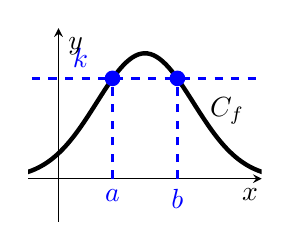
\begin{tikzpicture}[scale=1]
\begin{axis}[
axis x line=bottom,
axis y line = left,
axis lines=middle,
width=0.375*\linewidth,
height=0.333*\linewidth,
xmin=-0.5, xmax=4.5,
ymin=-1, ymax=4,
enlargelimits={abs=0.2},
xlabel={$x$},
ylabel={$y$},
%ytick distance=1,
ticks=none,
grid style=dashed,
%axis equal,
legend pos=north east,
xlabel style={at={(ticklabel* cs:0.95)},below=0.1},
]
\addplot[samples=101,smooth,ultra thick,domain=(-2:5),mark=none]{3.5*e^(-0.4*(x-2)^2)} node [pos=0.75,right] {$\mathscr C_f$};

\addplot +[mark=none,color=blue,style=dashed,very thick] coordinates {(-1,2.8) (5, 2.8)} node [pos=0.18,above right] {$k$};
\node[circle, minimum size=1pt,fill,color=blue,inner sep=2pt] at (axis cs:1.25,2.8) {};
\node[circle, minimum size=1pt,fill,color=blue,inner sep=2pt] at (axis cs:2.75,2.8) {};
\addplot +[mark=none,color=blue,style=dashed,very thick] coordinates {(1.25,0) (1.25, 2.8)} node [pos=0,below] {$a$};
\addplot +[mark=none,color=blue,style=dashed,very thick] coordinates {(2.75,0) (2.75, 2.8)} node [pos=0,below] {$b$};
%\addplot +[mark=none,color=red,style=dashed,very thick] coordinates {(-1, 0) (-1, 2)};
%\addplot +[mark=none,color=red,style=dashed,very thick] coordinates {(-1, 2) (0, 2)};
%\node[label={0:{$(0,1)$}},rectangle,fill,inner sep=2pt] at (axis cs:0,1) {};
%\node[label={[label distance=2pt]-90:{$(0,1)$}},rectangle,fill,inner sep=0pt, minimum height=0pt, minimum width=4pt] at (axis cs:1,1) {};
\end{axis}
\end{tikzpicture}}
&
\Centering{
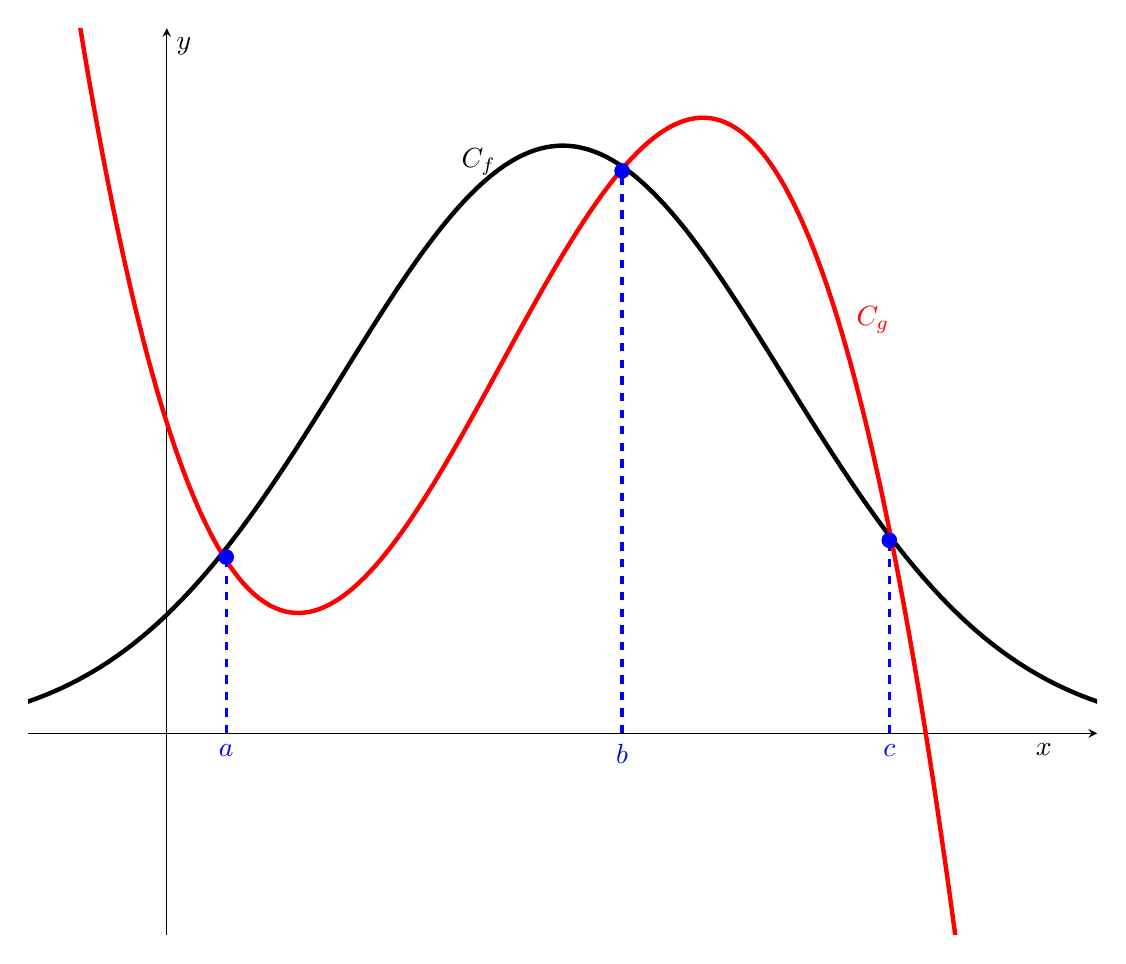
\begin{tikzpicture}[scale=1]
\begin{axis}[
axis x line=bottom,
axis y line = left,
axis lines=middle,
width=1.25*\linewidth,
height=1.08*\linewidth,
xmin=-0.5, xmax=4.5,
ymin=-1, ymax=4,
enlargelimits={abs=0.2},
xlabel={$x$},
ylabel={$y$},
ticks=none,
%ytick distance=1,
%axis equal,
yticklabel=\empty,
xticklabel=\empty,
xlabel style={at={(ticklabel* cs:0.95)},below=0.1},
]
\addplot[samples=101,smooth,ultra thick,domain=(-2:5),mark=none]{3.5*e^(-0.4*(x-2)^2)} node [pos=0.5,above] {$\mathscr C_f$};
\addplot[samples=101,smooth,ultra thick,domain=(-2:5),mark=none,color=red]{-0.69*x^3+3.49*x^2-3.72*x+1.85} node [pos=0.65,above right,color=red] {$\mathscr C_g$};

\addplot +[mark=none,color=blue,style=dashed,very thick] coordinates {(0.3,0) (0.3, 1.05)} node [pos=0,below] {$a$} node[pos=1,circle, minimum size=1pt,fill,inner sep=2pt] {};
\addplot +[mark=none,color=blue,style=dashed,very thick] coordinates {(2.3,0) (2.3, 3.35)} node [pos=0,below] {$b$} node[pos=1,circle, minimum size=1pt,fill,inner sep=2pt] {};
\addplot +[mark=none,color=blue,style=dashed,very thick] coordinates {(3.65,0) (3.65, 1.15)} node [pos=0,below] {$c$} node[pos=1,circle, minimum size=1pt,fill,inner sep=2pt] {};
%\addplot +[mark=none,color=red,style=dashed,very thick] coordinates {(-1, 0) (-1, 2)};
%\addplot +[mark=none,color=red,style=dashed,very thick] coordinates {(-1, 2) (0, 2)};
%\node[label={0:{$(0,1)$}},rectangle,fill,inner sep=2pt] at (axis cs:0,1) {};
%\node[label={[label distance=2pt]-90:{$(0,1)$}},rectangle,fill,inner sep=0pt, minimum height=0pt, minimum width=4pt] at (axis cs:1,1) {};
\end{axis}
\end{tikzpicture}}
\\ \hline
Résoudre l'inéquation $f(x)>k$ signifie trouver les nombres qui ont une image supérieure à $k$.

Cela revient donc à chercher l'abscisse des points de la courbe se situant "au dessus" de la droite d'équation $y=k$.

Ici, l'ensemble des solution de l'inéquation est:$$S=\left] a;b \right[$$ \vspace{-5mm}
&
Résoudre l'inéquation $f(x) \leq k$ signifie trouver les nombres qui ont une image inférieure à $k$.

Cela revient donc à chercher l'abscisse des points de la courbe se situant "en dessous" de la droite d'équation $y=k$.

Ici, l'ensemble des solution de l'inéquation est:$$S=\left] - \infty;a \right] \cup \left[ b ; + \infty \right[$$ \vspace{-5mm}
&
Résoudre l'inéquation $f(x) > g(x)$ signifie trouver les nombres dont l'image par $f$ est supérieure à l'image par $g$.
Cela revient à chercher l'abscisse des points de $\mathscr C_f$ situés "au dessus" des points de $\mathscr C_g$.

Ici, l'ensemble des solutions de l'inéquation est:$$S=\left] - \infty;a \right[ \cup \left] b ; c \right[$$ \vspace{-5mm} \\ \hline
\end{tabularx}
\end{center}
\end{methode}

\begin{exs}
\begin{center}
\begin{tabularx}{\linewidth}{|Y|Y|Y|} \hline
\begin{tikzpicture}
\begin{axis}[
styleglobal,
width=0.9*\linewidth,
xmin=-5, xmax= 5,
ymin=-2, ymax=5,
xtick distance=1,
ytick distance=1,
minor x tick num=0,
minor y tick num=0,
%tick label style = {font=\scriptsize},
]
\addplot[styleplot] plot coordinates {(-4,2) (-2,-1) (0,0) (2,3) (4,1.5)};
\end{axis}
\end{tikzpicture}
&
\begin{tikzpicture}
\begin{axis}[
styleglobal,
width=0.9*\linewidth,
xmin=-2, xmax= 8,
ymin=-2, ymax=5,
xtick distance=1,
ytick distance=1,
minor x tick num=0,
minor y tick num=0,
%tick label style = {font=\scriptsize},
]
\addplot[styleplot] plot coordinates {(-1,4) (4,2) (5,4) (7,-1.5)};
\end{axis}
\end{tikzpicture}
&
\begin{tikzpicture}
\begin{axis}[
styleglobal,
width=0.9*\linewidth,
xmin=-2, xmax= 8,
ymin=-2, ymax=5,
xtick distance=1,
ytick distance=1,
minor x tick num=0,
minor y tick num=0,
%tick label style = {font=\scriptsize},
]
\addplot[styleplot] plot coordinates {(-1,4) (1,2) (4,1) (6,4) (7,2)} node[pos=0.9,above right] {$\mathscr C_{h_1}$};
\addplot[styleplot,color=blue,densely dashed] plot coordinates {(-1,1) (3,4) (7,1)} node[pos=0.5,above right] {$\mathscr C_{h_2}$};
\end{axis}
\end{tikzpicture}
\\ \hline
Résoudre $f(x) \leq 1$:
\rule[-1cm]{0pt}{1cm}
&
Résoudre $g(x)>1$:
\rule[-1cm]{0pt}{1cm}
&
Résoudre $h_1(x) \geq h_2(x)$:
\rule[-1cm]{0pt}{1cm} \\ \hline
\end{tabularx}
\end{center}
\end{exs}

\rem{Exos Hyperbole}
\renewcommand\tabularxcolumn[1]{m{#1}}
\section{Etude du signe}

\begin{methode}
Dresser le tableau de signes d'une fonction $f$, c'est indiquer sur quels intervalles la fonction est négative, positive ou nulle.

Avec la même fonction que précédemment, on obtient:

\begin{center}
\begin{tikzpicture}
\tkzTabInit[lgt=1.4,espcl=2]{$x$/1,$f(x)$/1}{$-2$,$-1$,$2$,$5$}
\tkzTabLine{,+,z,-,z,+,}
\end{tikzpicture}
\end{center}

\end{methode}

\section{Parité d'une fonction}

\begin{defin}
Soit $f$ une fonction définie sur un intervalle $I$ centré en $0$ ( $I=[-a;a]$, $]-a;a[$ ou $\R$). On dit que f est:
\begin{itemize}
\item \textbf{paire} lorsque pour tout $x \in I, f(-x)=f(x)$.
\item \textbf{impaire} lorsque pour tout $x \in I, f(-x)=-f(x)$.
\end{itemize}
\end{defin}

\begin{exs}
\begin{itemize}
\item La fonction $\fonction f {[-2;2]} {\R} x {x^2-1}$ est paire car pour tout $x \in [-2;2], f(-x)=(-x)^2-1=x^2-1=f(x)$.
\item La fonction $\fonction g {]3;3[} {\R} x {0.5x}$ est impaire.
\end{itemize}
\end{exs}

\begin{proprs}
\begin{itemize}
\item $f$ est paire si et seulement si $\mathscr C_f$ est symétrique par rapport à l'axe des ordonnées.
\item $f$ est impaire si et seulement si $\mathscr C_f$ est symétrique par rapport à l'origine du repère $(0;0)$.
\end{itemize}

\begin{center}
\begin{tikzpicture}
\begin{axis}[
styleglobal,
width=0.9*\linewidth,
xmin=-6, xmax=6,
ymin=-1.5, ymax=3,
]
\addplot[styleplot]{0.25*x^2-1} node [pos=0.75,right] {$\mathscr C_f$};
%\addlegendentry{$f(x)=x^2-1$};
\addplot[styleplot,color=DarkRed]{0.25*x} node [pos=0.85,below right] {$\mathscr C_g$};
%\addlegendentry{$g(x)=0.5x$};

\end{axis}
\end{tikzpicture}
\end{center}
\end{proprs}

\begin{rmq}
Une fonction peut être ni paire ni impaire!
\end{rmq}

\begin{deroule}
\item \textbf{Total: 4 semaines}
\item Semaine 1
\begin{itemize} 
\item 1h30 - Activité intro ( coordonnées points, graphes )
\item 30m - Début du cours: I
\end{itemize}
\item Vacances - Semaine 2  
\begin{itemize}
\item 30m - Activité Emmanuel (remise en marche) - Questions 1 à 8
\item 3h - Cours II puis Exos 1 -> 8  (TD Chingatome en +)
\end{itemize}
\item Semaine 3
\begin{itemize}
\item 2h30 - Cours (in)equations + Exos Hyperbole
\item 1h30 - Cours Signe + Exos
\item 1h30 - Parité
\end{itemize}
\end{deroule}

\end{document}
